\chapter{Introduction}
\label{chapter:intro}


Cloud Computing can be defined as a new style of computing that has transformed a large part of the IT industry by allowing companies to build applications delivered as services over the Internet without making big capital investments. 
Thus these companies do not need to have their own datacenters. The initial financial requirements of running new IT services have been significantly reduced, besides the fact that companies do not need to be concerned about usage statistics, amount of resources, peak usage or about over/under provisioning. All of these features are possible thanks to Cloud Providers, companies that sell computing resources on demand, with a pay-as-you-go billing system. Such an approach to selling computing as a utility similar to how water or electricity is being sold is known as Utility Computing.
\par
Cloud Providers allow new ideas for business to grow up easier, breaking the past barrier of having to own a big datacenter and facing its capital expenses. They are companies that sell computer resources such as storage, CPU time, network traffic, applications and other services of their datacenters as an on-demand service. A Cloud is a net-worked pool of datacenter hardware and software that is shared among many users \cite{fox2009above}.
\par
Cloud Computing is defined by National Institute of Standards and Technology (NIST) \cite{mell2011nist} as a "model for enabling ubiquitous, convenient, on-demand network access to a shared pool of configurable computing resources (e.g., networks, servers, storage, applications, and services) that can be rapidly provisioned and released with minimal management effort or service provider interaction. This cloud model is composed of five essential characteristics:
\begin{enumerate}
\item On-demand self-service
\item Broad network access
\item Resource pooling
\item Rapid elasticity
\item Measured service
\end{enumerate}
It is offered in three different service models:
\begin{enumerate}
\item Software as a Service (SaaS)
\item Platform as a Service (PaaS)
\item Infrastructure as a Service (IaaS)
\end{enumerate}
And it has four deployment models: 
\begin{enumerate}
\item Private cloud
\item Community cloud
\item Public cloud
\item Hybrid cloud 
\end{enumerate}
We explain these terms below.

\bigskip

Typically, conventional (private) datacenters have a really low CPU load compared with their total resources, they are underutilized (average server utilization varies from 5\% to 20\% \cite{lynch2008cloud}). This is because companies do not just deal with their average work load, but also need to have capacity to also handle peak loads. Hence, new Internet companies managing their own datacenters have to pay beyond the resources they are going to need. Therefore Cloud Providers can become highly competitive in this scenario. They can offer what the company needs, neither more nor less, with the big advantage of costumers only paying for the resources they use, regardless of how much peak demand they will have to deal with.
\par
This type of rapid provisioning of resources for scale out and rapid releasing them for scale in is called elasticity and it is possible because of the huge amount of resources Cloud Providers have. 
All of these resources are available through standard protocols for all kinds of different client platforms.
 \par
In terms of who owns and manages the cloud, we find four types of clouds (Deployment models) defined by Jin, Hai, et al. in the "Handbook of Cloud Computing - Cloud types and services" \cite{jin2010cloud}:
\begin{enumerate}
\item Public Cloud: 
This is the most common type of cloud deployment, in which services and infrastructure are available to the general public on the basis of a pay-as-you-go policy or even free of charge. Both individual users and enterprises use these services over the Internet from a third-party provider sharing computing resources with the rest of its customers. Main public cloud vendors are Amazon AWS, Google and Microsoft.

\item Private Cloud:
Type of cloud where cloud infrastructure is operated solely for a single organization. Private Clouds are used internally, which means within the organization bounds. Private clouds are the choice for these large organizations or government departments who must have total control over the data they manage, achieving a more secure environment. 

\item Hybrid Cloud:
It is the composition of two or more previous cloud deployment types: Private and Public Clouds. The private cloud is able to scale out resorting to external resources provided by the public cloud to handle hardware failures, peaks usage or any other kind of temporal needs. Hybrid clouds allows organizations to keep their vital data and applications within organization bounds and use public clouds to host less vital data or applications.

\item Community Cloud:
This idea is derivated from the Grid Computing and Volunteer Computer paradigms. The idea is to share infrastructures between several organizations with similar requirements, allowing them to scale if needed while spreading the cost over the organizations \cite{wiki:cloud}.
\end{enumerate}


Cloud Providers offer resources of three different types: In \textbf{SaaS}, the Provider offers users applications ready to use, running on their cloud infrastructure. Users do not manage anything related to the infrastructure they are using (network, servers, storage, etc). In \textbf{PaaS}, users are able to deploy onto the cloud or use applications created using tools provided by the Cloud Provider (programming languages, services, libraries). Once more, users have not control over the used infrastructure. Finally, in \textbf{IaaS}, users control a big part of the cloud infrastructure that has been given to them, being able to deploy and run arbitrary software applications, different operating systems, and to control storage, host firewalls and related networking components.



\section{Cloud providers}

\begin{figure}[htb]
\centering
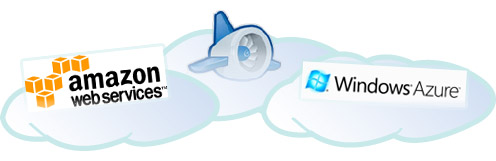
\includegraphics[width=0.8\textwidth]{./images/clouds.jpg}
\caption{Amazon Web Services, Google Cloud and Microsoft's Azure Services: the Cloud providers leaders} \label{fig:bigData}
\end{figure}


There are many cloud computing companies. Amazon and Google are two major players in this field, in which they offer Amazon Web Services (AWS) and Google Cloud Platform (GCP) cloud platforms, respectively. In order to have a more clear view of the actual Cloud landscape, we proceed to explain these two big cloud solutions, among some others in the following paragraphs.

\subsection{Amazon}
Since 2002, Amazon has been providing Cloud resources under the name Amazon Web Services \cite{amazon:aws}. AWS is a Cloud Computing Platform that offers scalable computing resources over the Internet. Amazon states that their users can have these resources up and running within minutes. AWS's offerings are accessed over HTTP, using REST and SOAP protocols. The communication with AWS is done through various web tools, browser plugins and standalone applications that provide an interface to AWS. Also this can be done using the Application Programming Interface (API) Amazon provides and integrating it into users' applications.

\bigskip
List of Amazon Web Services (related to this Thesis) \cite{amazon:aws}
\begin{enumerate}
\item Compute:
\begin{enumerate}
   \item Amazon Elastic Compute Cloud (EC2) is the Amazon IaaS solution. It provides scalable virtual machine based computation environments using the Xen Hypervisor \cite{Xen} to manage their Amazon Machine Image (AMI) instances. This server instances can be set up and booted within minutes, scaling their capacity according to computing requirements changes through a simple web interface. Amazon EC2 provides users with total control of their computing resources. 
   \item Amazon Elastic MapReduce (EMR) allows businesses, researchers, data analysts, and developers to easily and cheaply process vast amounts of data. It uses a hosted Hadoop framework running on the web-scale infrastructure of EC2 and Amazon S3.
\end{enumerate}
\item Storage  \& Content Delivery:
\begin{enumerate}
 \item Simple Storage Service (S3) provides Web Service based storage.
\item Amazon Glacier, Provides a very low cost long-term storage option (when compared to its S3 service). High redundancy and availability, but very long access latency. Ideal for archiving data.
\item AWS Storage Gateway is an iSCSI block storage virtual appliance with cloud-based backup.
\item Amazon Elastic Block Store (EBS) provides persistent block-level storage volumes for EC2.
\end{enumerate}
\item Database:
\begin{enumerate}
\item Amazon DynamoDB provides a scalable, low-latency NoSQL online Database Service backed by Solid State Disks (SSDs).
\item Amazon ElastiCache provides in-memory caching for web applications. This is Amazon's implementation of Memcached.
 \item Amazon Relational Database Service (RDS) provides a scalable database server with MySQL, Oracle, and SQL Server support.
 \item Amazon Redshift provides petabyte-scale data warehousing with column-based storage and multi-node compute.
\item Amazon SimpleDB, allows developers to run queries on structured data. It operates in concert with EC2 and S3 to provide "the core functionality of a database."
\end{enumerate}
\item Deployment
\begin{enumerate}
\item AWS Elastic Beanstalk provides quick and easy deployment and management of applications in AWS cloud. It is the main Amazon's PaaS solution. Elastic Beanstalk harnesses AWS services to complete its task successfully. Elastic Beanstalk takes care of the application's deployment: capacity provisioning, load balancing request, automatic scaling, etc. It supports Node.js, PHP, Python, Ruby, .NET and Java. 
\end{enumerate}
\end{enumerate}

Amazon Web Services is used by many cloud companies to provide new cloud services, including RightScale providing IaaS, Heroku providing PaaS or Dropbox providing SaaS.

\subsection{Google}

Google infrastructure has been built and continues being built to work on datacenters of commodity hardware as opposed to high-end hardware due to what is called the economy of scale: costs are reduced and overall computing power is maximized. Google has managed to develop a fault-tolerant elastically scalable system to work on several datacenters of commodity hardware, letting them to offer cheap Cloud Services.
\par
With that premise, Google entered the Cloud Computing business in 2008 with the Google App Engine offering. Whilst cloud provisioning is not their core business, they have given to the world numerous and important contributions in this field.
Google App Engine (GAE) is Google's PaaS solution. GAE allows users to host and run web applications and store data in Google-managed datacenters distributed around the world. It supports Java, Python, PHP and Google's Go programming languages. Users develop their applications on their local machines before uploading the applications to GAE. Then, it is GAE who takes care of the provisioning and deployment of the application uploaded on the infrastructure. Also automatic scaling is done during the life of the deployed application. Users do not need to keep an eye on the servers as this is GAE infrastructure's job. GAE software development toolkit (SDK) is provided by Google in order to allow users to develop their solutions in a simulated GAE's environment. Google also supplies APIs that can be used to integrate Google services with developer applications.
\par
On June 2012, Google announced Google Compute Engine (GCE) [cite] at Google IO. GCE is Google's IaaS solution. GCE allows users to run large-scale CPU works on Linux virtual machines hosted on Google's infrastructure. GCE provides all resources through the Google APIs Console, a collection of Google's APIs. GCE is very similar to Amazon's EC2 solution, both provides scalable CPU capacity. 
After that, Google unified its cloud solutions under the name of Google Cloud Platform (GCP) \cite{CloudGoogle}. 
\par
Google Apps \cite{GoogleApps} is the Google's SaaS implementation launched on 2006 and entirely based on Google's own infrastructure. It is a set of several Web applications which offer an online alternative to traditional offline office software. But Google Apps is not just an online office suite, but also a solution that allows users to communicate and collaborate between their projects easily. With Google Mail users can communicate with emails, online messaging and voice or video calls. Thanks to Google Docs users can create, edit, delete their documents, spreadsheets or slides. Google Calendar is a powerful online calendar application. Google Web Pages allows for publication Web pages. Google Drive offers file storage and synchronization to users. Recently, in the Google IO 2013 meeting, Google added to their Google Apps collection Google Hangouts. It creates online video meetings with a click, allowing users to work with clients or partners in real time.
\par
The main advantage of Google Apps is that everything is online, users do not need to install any software locally, they just need a computer with Internet connection and a Web browser to interact with Google Apps.

\subsection{Microsoft}

When analyzing this field, Microsoft has always something to offer. Windows Azure \cite{Azure} is Microsoft's platform for Cloud Computing. It was announced at the Professional Developers Conference in October 2008,  and commercially available since February 2010. In the beginning, Windows Azure supported only .NET development. However, now it supports many different programming languages, tools and systems, not only Microsoft-specific ones, but also third-party tools, such as Java, Ruby, PHP, Node.js and C++. Windows Azure is hosted in Microsoft-managed datacenters distributed around the world. Microsft states that Windows Azure enables users to deploy their applications within minutes and scale in/out them to any size in a fully automated way.
Windows Azure provides an API built on REST, HTTP, SOAP and XML that allows users to communicate with Windows Azure services easily. Microsoft also provides open-source Windows Azure client libraries for multiple programming languages. These SDKs help users build, deploy and manage their Windows Azure applications.
\par
Nowadays, Windows Azure Platform offers Infrastructure as a Service (IaaS) features that complement their initial offering of PaaS features. The Azure platform provides three distinct computing service models \cite{Azure:description}:
\begin{enumerate}
\item Windows Azure Web Sites, which is their PaaS service for Web hosting. Users can create web sites in PHP, .NET, Python and Node.js and deploy them using git, FTP or TFS. Web Sites supports horizontal scalability of web sites, from shared single instances to dedicated large instances.
\item Windows Azure Cloud Services, the traditional Microsoft PaaS service offering. Cloud Services are containers of hosted applications. Applications execute in virtual machines, also called instances, running Windows Server OS. Windows Azure itself manages the instances. Cloud Services allows to create scalable and reliable applications.
\item Windows Azure Virtual Machines, which comprises the Microsoft IaaS solution for their public cloud. Users create Virtual machines on demand. Unlike Windows Azure Cloud Services, users have total control of their created virtual machines. The Virtual machines offering includes Windows Server images as well as Linux distributions images provided by Microsoft partners.
\end{enumerate}

Windows cloud offerings are not just PaaS and IaaS solutions, but also SaaS tools. Windows Live is a Windows's SaaS which integrates search, email and a social network system. Skydrive is the cloud hosting Microsoft SaaS model. And Microsoft SharePoint is Microsoft collaborative cloud system, which allows multiple users to work together in real time.


\subsection{RackSpace}

Behind these three big players, RackSpace \cite{RackSpace} is one of the strongest cloud providers companies. Powered by an offering mostly based on the OpenStack Cloud Computing platform, Rackspace is a mostly open source based alternative to Amazon, Google and Windows Azure. One of its strengths is its ability to roll out the latest Openstack features, thus continuosly improving its functionality. Rackspace offers three different Cloud Services: Cloud Servers, their IaaS solution, Cloud Sites, which is their PaaS solution, and Cloud Files for storing files in the cloud, which is their SaaS solution. 
\par
As Eric Savitz states in a Forbes article \cite{Rackspace:forbes}, in the last quarter of 2012, Rackspace total server amount has increased from 89.051 to 90.524, along with an increase of their total customers from 197.635 to 205.538.

\section{Behind the big Cloud providers}

Nowadays Amazon, Google, Microsoft are the biggest Cloud providers over the world, but this does not mean there are no other competitors offering excelent products in the Cloud field. Here we show the most promising cloud providers categorized by their offerings of resources: IaaS, PaaS and SaaS.

\subsection{IaaS}

Infrastructure as a Service cloud segment accounted for the majority of total market revenue in 2012 with more than half of the total public cloud market share \cite{aslett2013451}. The main responsibles for this impressive market quota are Google with its Google Cloud Platform, Amazon and Microsoft Azure, all of them deeply studied in the previous section 1.1. 


\subsection{PaaS}
Among the subcategories of Cloud Computing, the Paas layer is experiencing a fast growth. According to the Market Monitor research report \cite{aslett2013451}, PaaS accounted for the 24\% of the total public cloud revenue in 2012 and it is expected to grow between 2012 and 2016 at a 41\% compound annual growth rate (CAGR). Many companies are behind this success, in the following lines we describe some of them.
\par
Heroku \cite{heroku} is a cloud Platform as a Service (PaaS). It has been in development since 2007, what makes Heroku one of the original PaaS offerings in the world. Nowadays it is owned by Salesforce.com since 2008. At the beginning, Heroku supported only the Ruby programming language, but since then, Heroku has been adding support for more programming languages: Java, Scala, Python, Node.js, Clojure, Grails, Gradle, Play and PHP. Heroku platform is entirely based on the AWS EC2 and S3, giving it the ability to scale in/out to satisfy customers' demands.
According to former Heroku CEO Byron Sebastian, Heroku was hosting more than 1.5 millions applications by November 2010 \cite{Heroku:gigaom}.
\par
Openshift \cite{OpenShift} is another interesting and new cloud PaaS product offered and developed by Red Hat. OpenShift is free and open-source, although now it has a paid version which adds extra support and features. The software that runs the service is called OpenShift Origin \cite{OpenShiftOrigin} and can be downloaded from Github, allowing users to change it according to their needs.OpenShift is aimed at Java, Python, PHP, Node.js, Perl and Ruby developers and, as many others PaaS, OpenShift is based on AWS, this one specifically in Amazon EC2.
\par
CloudBees \cite{CloudBees}
% \cite {http://www.infoworld.com/d/cloud-computing/which-freaking-paas-should-i-use-204189?page=0,2#paas2} %\cite{http://gigaom.com/2011/07/25/3-paas-lessons-from-cloudbees-funding/}
offers a Java-based PaaS to host, run and manage Java applications. It is one of the first PaaS aimed mainly at the Java developer. CloudBees supports any JVM-based programming language or framework. Jenkins Continous Integration (CI) tool is included in the CloudBees PaaS. It supports developers through the whole application life cycle directly in the cloud from Github. The CloudBees service provides middleware on top of some public cloud, such as Amazon Web Services, OpenStack and VMware vSphere though customers can also run the service on private cloud infrastructure.

\subsection{SaaS}
Software as a Service layer also strikes strongly in the Cloud race. SaaS represented 25\% of total cloud revenue in 2012 and it is expected to follow growing in the following years \cite{aslett2013451}. In the next paragraphs, we highlight two successful SaaS companies without forgetting Google SaaS products Google Apps and Windows SaaS offerings previously described.
\par
Talking about successful SaaS solutions, we always find Dropbox \cite{Dropbox}. Dropbox is a SaaS solution developed by Dropbox Inc., and launched on September 2008, that offers cloud storage and file synchronization to users. Dropbox uses Amazon S3 to store all files. 
In a fact sheet \cite{Dropbox:sheet} released in March 2012, Dropbox stated that they had over 50 million users, and nine months later, in November 2012, Dropbox announced that they had over 100 million users \cite{Dropbox:thanks}.
\par
Another notable SaaS is Salesforce.com \cite{Salesforce.com}, which is one of the most popular SaaS Customer Relationship Management (CRM) platform. It offers on-demand CRM services for all kind of organizations. Salesforce.com presents two major products. Sales Cloud is a set of applications to manage sales, customers and other business activities more easily and efficiently; and Service Cloud, which provides organizations with a community help-desk.
\par
Unlike Dropbox or many other SaaS solutions, Salesforce.com is built on its own infrastructure: Force.com \cite{Force.com}, which is the Salesforce.com's PaaS product.


\section{Big Data}


Until now, we have showed the three most popular cloud paradigms: Infrastructure as a Service (IaaS), Platform as a Service (PaaS), and Software as a Service (SaaS) and how Google, Amazon, Microsoft and Rackspace among other companies offer their Cloud Services. Now it is time to move to one problem that has born with the outbreak of the Cloud Computing.
\par
Thanks to the features that Cloud Computing has brought with itself (pay-on-demand, elasticity, etc), lot of new applications have seen the light. Thanks to the new cloud business, they are now economically viable and before not. More and more novel applications harness the Cloud Computing paradigm every day, which means a never seen increase in the amount of generated as well as consumed data, called Big Data. Thus, scalable Database Management Systems (DBMS) have become a fundamental and critical part of cloud infrastructures \cite{agrawal2010big}.

\begin{figure}[htb]
\centering
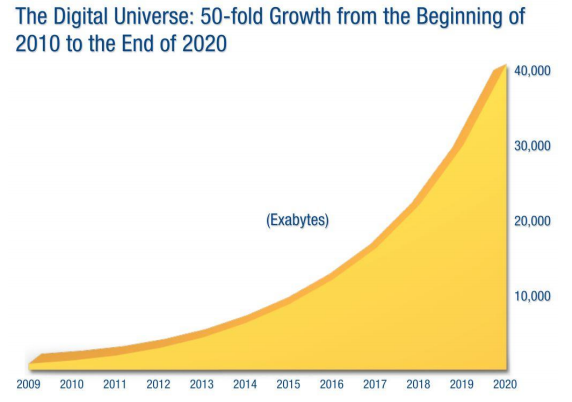
\includegraphics[width=0.8\textwidth]{./images/bigData.png}
\caption{Growth of data from the beginning of 2010 to 2020. Figure extracted from IDC's Digital Universe Study, December 2012} \label{fig:bigData}
\end{figure}

Figure 1.X depicts how fast generated data is growing. International Data Corporation (IDC) estimates that by 2020, the digital universe will grow to 40,000 exabytes, in more understandable words, 40 trillion gigabytes. From now until 2020, the generated data will double every two years \cite{gantz2012digital}.

Google has been one of the first companies that has addressed the Big Data problem, which is handling large amounts of data. Google has designed its own MapReduce programming paradigm \cite{dean2008mapreduce}, allowing them to do scalable distributed batch processing of large amounts of data: Web request logs, crawled documents, etc. Related to this field, Google designed and implemented their own distributed file system to be used in combination with their MapReduce framework, which was called Google File System (GFS) \cite{ghemawat2003google}. These are systems designed to run on a large cluster of commodity machines and are highly scalable, but both implementations remain private to Google \footnote{Colossus is the new version of the GFS as mentioned in the Spanner paper on OSDI 2012 \cite{corbett2012spanner}}.
\par
After the publication of MapReduce and the GFS, Apache Hadoop \cite{ApacheHadoop} entered the scene as the open-source alternative to Google MapReduce and Google File System. Apache Hadoop is an Apache project that includes implementations of a distributed file system, namely Hadoop Distributed File System (HDFS)  \cite{white2012hadoop, shvachko2010hadoop}, and Hadoop MapReduce \cite{ApacheHadoop}, both inspired by Google projects. Hadoop was initially created in 2004 by Doug Cutting (and named after his son's toy elephant). In January 2008, Hadoop became a top-level Apache Software Foundation project. Nowadays it has many contributors, both academic and commercial (Yahoo being the largest commercial contributor), and continues growing.
\par
The field of distributed systems for Cloud Computing continued expanding, and as a logical next step, researchers needed a database for the applications to store the massive amount of data they were generating. Until then, the traditional and massive used Relational Databases Management Systems (RDBMS) have offered a simple and good solution according to the needs of the moment, but with the arrival of Web applications with massive numbers of users, the requirements of storage database systems for this new generation of applications have changed. Traditional databases did not offer a suitable and feasible storage solution to the new massive amount of data. In 2006, Google published a paper talking about BigTable \cite{chang2008bigtable}. Bigtable is a distributed storage system built on GFS for managing petabytes of structured data across thousands of commodity servers. Between its goals, we can find wide applicability, high performance, high scalability and high availability. To achieve such goals, BigTable uses a simple data model that supports dynamic control over data layout and format. Developers do not have to define a schema to store structured data, giving them a high flexibility when building applications. Albeit, such a simple data store brings with it a lack of characteristics. Lacking in particular are ACID transactions, Join operations and accessing through a natural query language like SQL that RDBMSes offer.
\par
As a response to BigTable we find Apache HBase \cite{ApacheHBase}, which is an open source project, modeled after Google's BigTable and written in Java. Developed as part of Apache Software Foundation's Apache Hadoop project, it became an Apache top-level project on 2010. Hbase uses HDFS as the underlying storage system for the created tables and the Apache ZooKeeper as a distributed coordination service, similar to the use of Chubby \cite{burrows2006chubby} in BigTable. Hbase features are similar to BigTable features; its implementation is very close to BigTable implementation with same properties. Main differences lie in implementation details. For example, how the memory is mapped or how the Garbage Collector works \cite {samar2011scalable}.
\par
HBase, BigTable and many others Cloud data stores are included in the group of so-called NoSQL databases \cite{NoSQLdatabases}. All of them are distributed storage systems mainly designed to offer a really good performance when dealing with Big Data, contrary to what traditional SQL databases do. 

\bigskip
\fixme{This thesis is structured as follows. In the next chapter, we present background knowdledge of ...... In chapter 3, we describe experiments....}
\bigskip


